\selectlanguage{English} %choose: ngerman or English
%%%%% Angaben f�r die Titelseite

% Titel der Arbeit
\Vtitle{Seminar MMI \\A Survey on Explainable Artificial Intelligence}
% Autor der Arbeit
\Vauthor{Si Hao Shen}
% e-mail des Autors
\Vaddress{si.hao.shen@rwth-aachen.de}
% Kurzfassung der Arbeit
\Vabstract{
	Artificial Intelligence (AI) has impacted the world and various fields of study enormously over the last few years. If developed with great care and appropriately, it is possible that the AI system may outperform human experts. However, the well developed AI system may be a complex function with opaque features that only a few of people can make sense of. To overcome the lack of explainability in such AI system, the responsibility falls into the research field of explainable AI (XAI). XAI provide accessible interpretations of how AI systems conduct their prediction and analysis. It is widely acknowledged, XAI as a crucial feature when deploying an AI model. Thus, the goal of this survey is to provide an overview with existing literature and ideas in the field of XAI, and also with a prospect of what opportunities and series of challenges lie ahead in the future of XAI.
}
% Schl�sselworte zum Inhalt der Arbeit
\Vkeywords{Explainable Artificial Intelligence, Interpretability, Fairness, Transparency, Responsible Artificial Intelligence}
% tats�chliche Erstellung der Titelseite
\makeArticleTitle


% Beispiel f�r einen Abschnitt

\section{Introduction}
\label{sec:CSorg}

\begin{center}\emph{"The fact that man cannot combine information as efficiently as a computer, for example, does not imply that man can be replaced by machines. It does imply that the necessity for a man-computer system is at hand."} \cite{einhorn}\end{center}


While Artificial Intelligence (AI) extract new information and provides incredible insight from data in various fields of study, it enables new possibilities and efficiencies at scale one cannot imaging. In order to achieve better performance, the capabilities of AI methods are becoming increasingly complex over time. To such that almost no human intervention is needed during its computation. However, when the prediction of such AI model may affect human lives in e.g. medicine, law and energy etc., the importance of the need for understanding how such prediction by AI model is made, is self-explaining. Thus the demand for transparency in black-box ML models has increased over the last few years. Figure 1 gives a quantitative look of the rising trend of XAI and related concepts with time on the x axis over number of total publications with title, abstract and/or keywords related to the field of XAI. 

\begin{figure}[htb]
	\centering 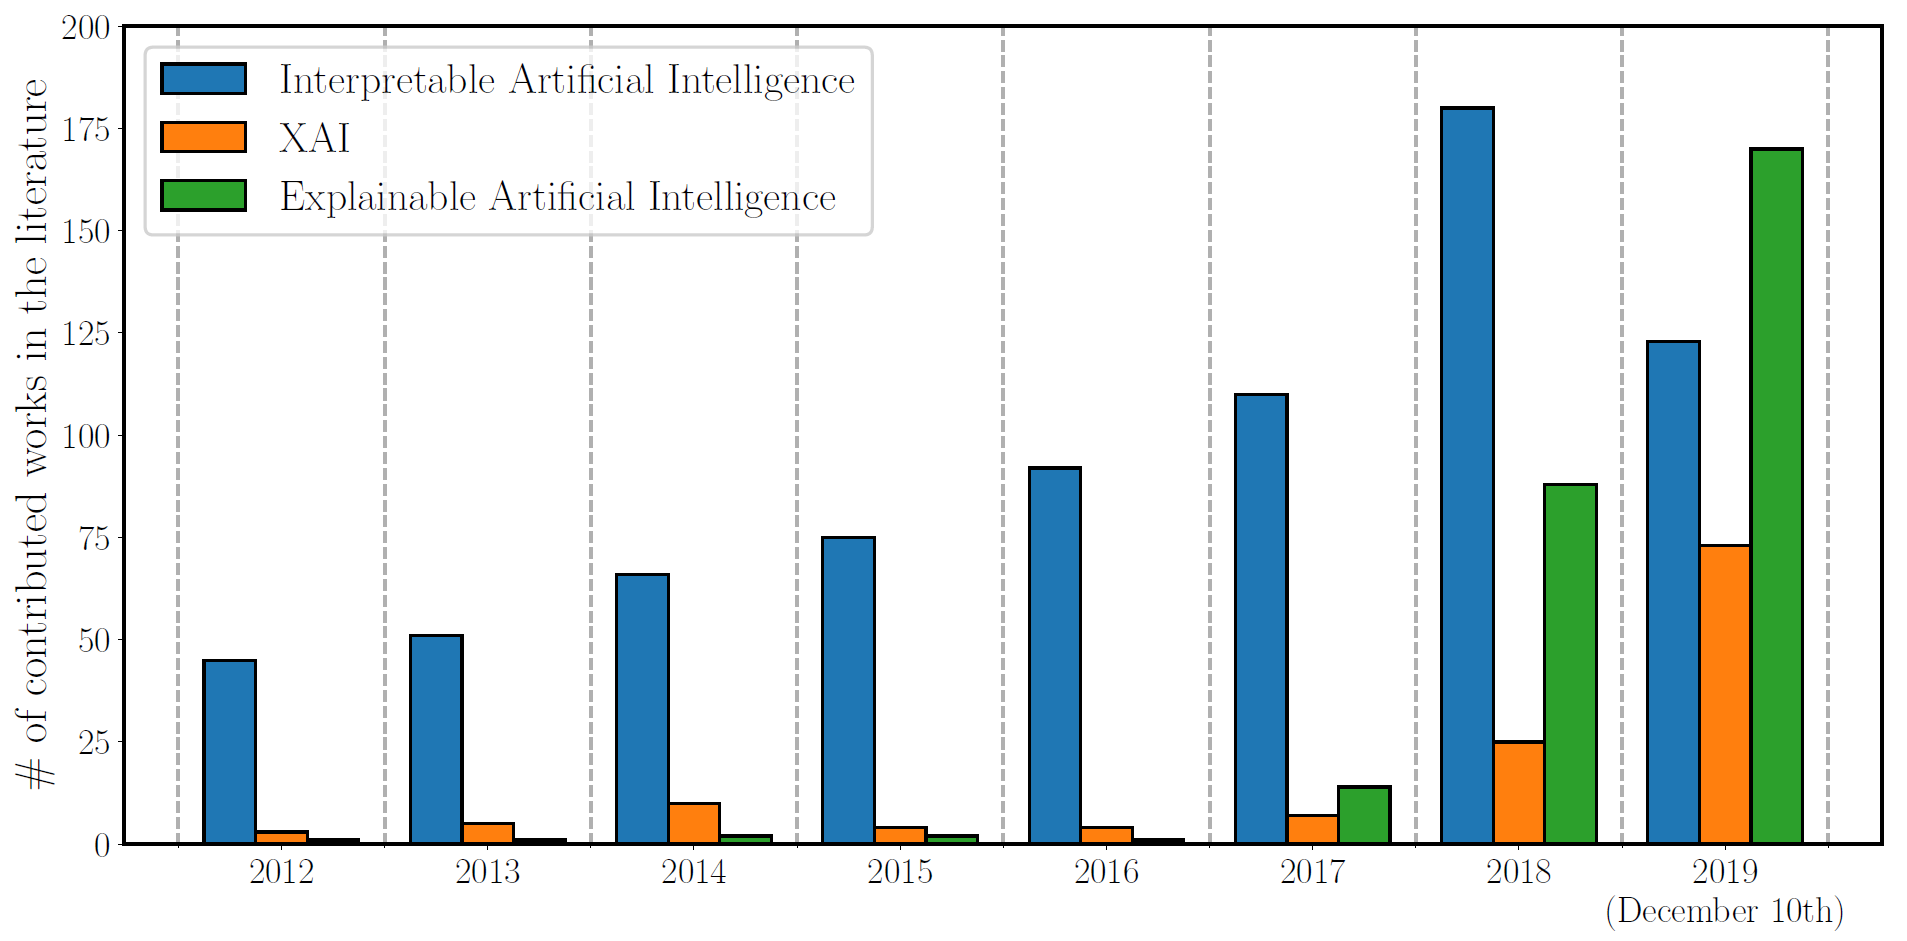
\includegraphics[width=1\textwidth]{bilder/Figure_1.png}
	\caption{Increasing trends and interests in the field of XAI, evaluated in numbers of total publication with title, keywords and abstract related in XAI over every year, data from Scopus \cite{aleja}.}
	\label{fig:Testbild}
\end{figure}

It is evident that developing XAI is necessary, there are 3 main reasons why the AI world needs to adapt XAI techniques into the black-box models:

\begin{itemize}
	\item \textbf{Empowering decision-making}: Explainability helps the developers and users in process of decision-making, it can detect bias and misleading prediction computed from the black-box model.
	\item \textbf{Additional Robustness}: By gaining Explainability, the black-box model can maintain more stable behavior, and can avoid errors that might have negative effect on the prediction beforehand.
	\item \textbf{Predictable behavior}: It also gives users an insurance and trust to the black-box system, that the prediction is made meaningfully by inferring the variables and features. An extra layer of reasoning can be obtained in the scope of explainability. 
\end{itemize}

That means in order to gain explainability in a black-box system, it is important to obtain an understanding of the model structures and predictions, a visualization of the abstract rules used in the model, or a hint on abnormality of such system, for the sake of robustness \cite{hall}.

The goal of this survey is to provide an overview of general concepts in XAI and to understand state-of-the-art XAI methods used in various fields of study. In section 2, a detailed definition of what XAI is given, and how are the other terminologies defined differently such as transparent AI, interpretable AI. A brief overview of available XAI techniques is also introduced. Furthermore, the need of XAI and how to apply an XAI system are discussed. Also, the limitations of XAI fall into this discussion. 

In section 3, a detailed look on the existing XAI methods is explained. Some machine learning methods are inherently interpretable, such as Bayesian models, linear regression, which falls into the category of transparent model. Other complex black-box model, such as Neural Network is not easy to explain, without sacrificing the performance accuracy and simplify the model architecture and reduce the number of hyperparameters. Thus, there are specific methods to describe such complex opaque model. One general technique is called post-hoc explainability technique, which uses explanation by simplification, local explanation, and visual explanation to give understandable information about the prediction of such model made. Further discussion about one of a specific post-hoc techniques is conducted, which is the hybrid modeling method. In short, it uses both the original and simplified transparent model in order to maintain the model performance and simultaneously gain insights and explanations into the complex black-box model. And finally, an overview of available XAI toolboxes and libraries is introduced. 

In section 4, a use case describes about how XAI is applied to a robotic arm and its task planning algorithm. The goal of this paper, is to let the robot learn about different interpretations that a human operator can conclude, while holding a cup or a knife, regardless both motion planning tasks are identical to the robot itself. It is named as explainable planning, which means the robot has two models one model from the human's perspective and the other from its own model, in order to compare the differences of these two models and gain human interpretation of such robot behavior.


In the last two sections, the principle of how to conduct an XAI system is introduced and what opportunities and challenges may come in the way when developing such system. Finally, the literature survey concludes with an outlook for the future of XAI and beyond XAI, namely the development of responsible AI, which adds more features besides explainability: such as fairness, data privacy, and accountability.

\section{XAI}
\subsection{Definition}

The first question is most often: What is explainable AI (XAI) exactly? As it is still in an early stage of XAI development, there exist many definitions contain somewhat ambiguous definitions and can be easily misunderstood and misinterpreted from the reader. That is why it is important to come-up with a detailed and exact definition of XAI as early as possible. There are many resources and great definitions being stated from different discipline, as from research, from industrial, as well as from government, such as quote:

\begin{center}\emph{"XAI will create a suite of machine learning techniques that enables human users to understand, appropriately trust, and effectively manage the emerging generation of artificially intelligent partners."} \cite{darpa}\end{center}

\begin{center}\emph{"Explainable Artificial Intelligence is a system that produces details or reasons to make its functioning clear or easy to understand."} \cite{aleja}\end{center}

\begin{center}\emph{"AI model should not only solve pattern recognition problems, but also provide causal models of the world that support explanation and understanding."} \cite{joshua}\end{center}

The above quotes share the same notion that by developing an XAI system, it should not be an opaque system, that only experts of the field can understand its complex mathematical formulas, but the output of XAI system should be interpretable and explainable. XAI should provide details or reasons to make its functioning clearly or easy to understand. In this sense, an reduction of complexity of the AI model as a \textbf{transparent model} or to simplify its outputs as \textbf{post-hoc explainable model} should be considered as an XAI approach. Note that most of XAI are actually explainable machine learning (ML), although AI is much more than machine learning.

There exist also various concepts which act like synonyms of XAI, such as fair AI, interpretable AI and transparent AI, but they do not share exactly the same notion. For which are stated as following:

\begin{itemize}
	\item \textbf{Fair AI}: It comes from a social standpoint to ensure that machine learning models don't reinforce biases and subsequently, they treat all different users fairly and equitably.
	\item \textbf{Interpretable AI}: This is the most similar terms for explainable AI. Interpretable AI is able to explain or provide meaning in human natural language, it gives a sense of understanding how the technology works to non-expert users. The Interpretable part can be build in to an XAI system regards to which target users the developer want to attract.
	\item \textbf{Transparent AI}: Gives a level of accessibility to the data used and algorithm implemented in the AI system. Just like interpretable AI, transparent AI can be included in an XAI system depending on the developer's application, but is not necessary. According to \cite{lipton}, there are three categories of transparent AI: simulatable model, decomposable model and algorithmically transparent model.
	\item \textbf{Explainable AI}: As defined earlier it enables a wide range of users to understand the conclusion of an AI system, the how and why the model makes this particular predictions and not others. This gives the user an interface between them and the AI system. 
\end{itemize}

Explainability is however a broad concept, depending on the various field of interest from different readers, it can mean entirely different. Thus it needs to be discussed more detailed in the next section: why do we need XAI? For what different purposes of explainability and degree of explainability do we need in our applications?

\subsection{Why XAI}
XAI can enable trust and confidence to the end users, however it needs to treat with caution, as these explanations can be seeming plausible but may mislead users about the effectiveness of the system. To avoid this kind of problems, developers need to know beforehand what their purposes are for developing XAI system and who are their target users. Following figure 2 listed a few purposes of XAI \cite{rossi}: 
\begin{figure}[htb]
	\centering 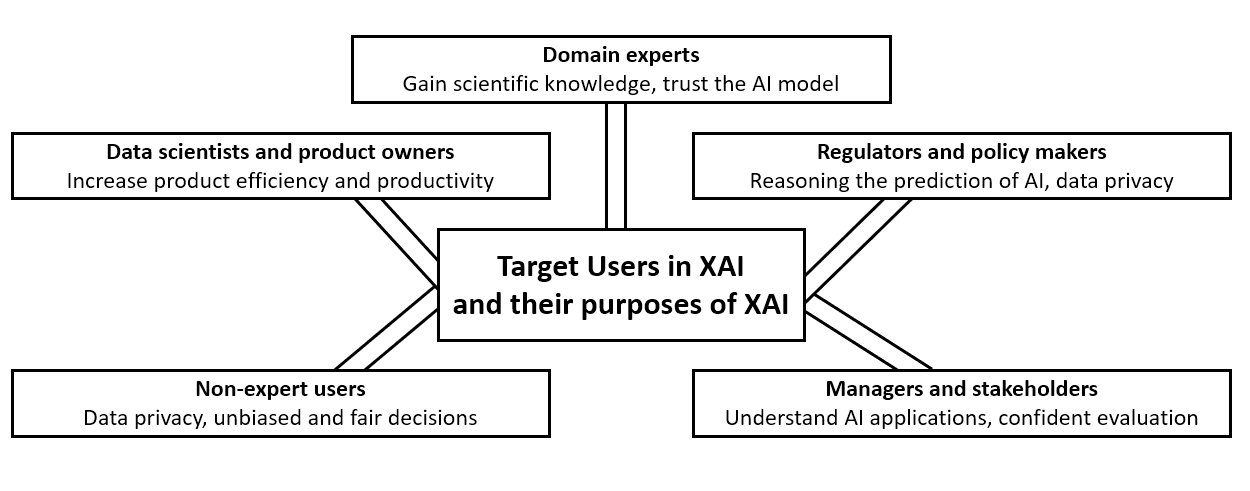
\includegraphics[width=1\textwidth]{bilder/Figure_2.png}
	\caption{Different purposes of XAI usage by different profiles from target users.}
	\label{fig:Testbild}
\end{figure}

\begin{itemize}
	\item \textbf{For domain experts}: e.g. medical doctors, scientific researchers need to trust the model, analysis the prediction the model made in order to gain scientific knowledge. Trust means that the model will act as intended to be given a well defined problem. The model should also provide explanations, a certain degree of causal relationships between the prior expert knowledge and the predicted ones, with causality inference techniques beyond correlation. 
	\item \textbf{For regulators and policy makers}: they need an AI model to be able to reason its own predictions confidently and is aware of data privacy. Nevertheless, fairness and non-discrimination need to be addressed as well as when it comes to decide effective and unbiased legislation and put it in force.
	\item \textbf{For data scientists and product owners}: they want to know how to ensure and improve product efficiency, research on the interests of their users to bring up new features and functionalities into their products. A certain degree of accessibility of the XAI model needs to be provided, in order to give them the freedom to modify the underlining algorithm, model structure etc. for their own use.
	\item \textbf{For managers and stakeholders}: similar to regulators and policy makers, they want to understand the causality of its prediction, with amount of confidence to assess and to evaluate in depth, how the regulation is going to effect the company.
	\item \textbf{For non-expert users}: mainly to understand how their data is processed and used by the model, privacy awareness is certainly important in this context. And also from a social standpoint, the predictions being made, need to be fair and unbiased toward the users. 
\end{itemize}

After describing the purposes and goals of various users might expect when using an XAI system, it is clear that XAI may contain different functions and meanings, thus performs entirely different from one discipline from another. In the next subsection, it is discussed broadly how can one apply XAI and which state of the art XAI methods already exist. In section 2, a more detailed survey of XAI methods focusing on machine learning (ML) model is discussed.

\subsection{How to apply XAI}
In literature, there are mainly two categories of XAI techniques, one is called \textbf{transparent model} and the other \textbf{post-hoc explainable model}. Transparent model means that the machine learning model is inherently interpretable and explainable by design. \cite{guidotti} It is classified further with 3 different level of transparency: algorithmic transparency, decomposability and simulatability, see figure 3.
\begin{figure}[htb]
	\centering 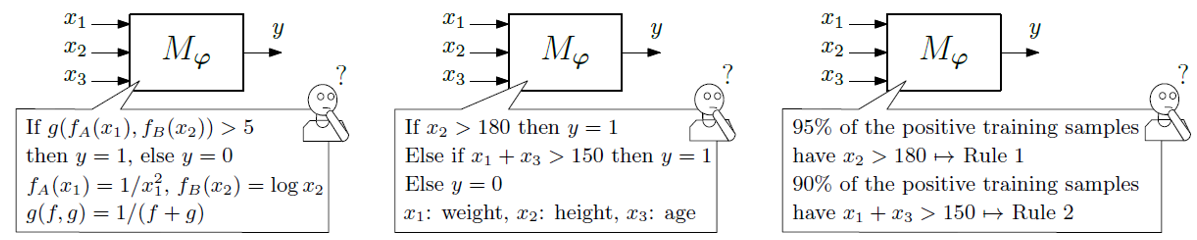
\includegraphics[width=1\textwidth]{bilder/Figure_3.png}
	\caption{Different level of transparency, from left to right: simulatability, decomposability and algorithmic transparency \cite{aleja}.}
	\label{fig:Testbild}
\end{figure}

Algorithmic transparency means that the process, in other word, the algorithm used to compute input into output is easily understandable for developers and users. For instance, linear model is algorithmic transparent, its prediction and error can be easily interpreted and analyzed. As contradiction, model with deep architecture e.g. deep neural network is an opaque system, thus its algorithm cannot be fully comprehensible even to its own developer. Its solution need to be approximated using optimization such as stochastic gradient descent.

\textbf{Decomposability} can explain every part of a model, regarding its model architecture, input, target, hyperparameters. It gives the users freedom of explaining and understanding the behaviour of a model. However, it is not easy to obtain as it requires every model input to be interpretable to human, which can be cumbersome and unnecessary depending on the usage of the model.

\textbf{Simulatability} is the properties of the system and its process can be simulated. In other words, when a model is simulatable, it means it is also algorithmic transparent and can be decomposed without difficulties. A simple 3 layer neural network with less than 10 perceptrons can be simulatable, whereas interpretable rule based system with large amount of rules is not.

\textbf{Post-hoc explainability techniques} are implemented in complex AI models, where they are not interpretable inherently, such as deep neural network. There are several existing explanation techniques to improve their interpretability: local explanations, text explanations, visual explanations, feature relevance explanations, explanations by example, explanations by simplification. 

\textbf{Local explanations} as the name suggested, gives explanations to less complex substructure of the whole model and only explain part of the system. \textbf{Text explanations} generate text in order to help explaining the predictions of the model \cite{bennetot}. \textbf{Visual explanations} aim to visualize the model's behavior using dimension reduction methods. \textbf{Feature relevance explanation} is an indirect method, which computes a sensitivity score system for its prediction and variables used in the AI model. Comparing the score can give user and developer a insight to how variable is sensitive toward predicted value and what variable has the largest impact to the prediction. \textbf{Explanations by example} give user representative data examples to analyze the correlation of the input and the prediction. And finally \textbf{explanations by simplification} extract and reduce the complex AI model to a simplified one and keeping a similar model performance. The Local Interpretable Model-Agnostic Explanations (LIME) uses such technique to explain predictions from a deep convolutional neural network \cite{ribeiro}

This subsection gives a taste on different approaches toward XAI techniques, a more extensive view and a detailed survey about XAI methods is discussed in section 2. 


\section{XAI Methods}
\subsection{Overview}
In the last section, it is discussed the different methods of XAI and shown there are two main categories: transparent models and post-hoc explainable models. Transparent models are inherently interpretable and understandable models and they can be explained without external explanations. Examples of models which falls into this category are logistic regression model, linear regression model, K-nearest neighbors, rule-based learners, general addictive model and bayesian model, see figure 4. 

\begin{figure}[htb]
	\centering 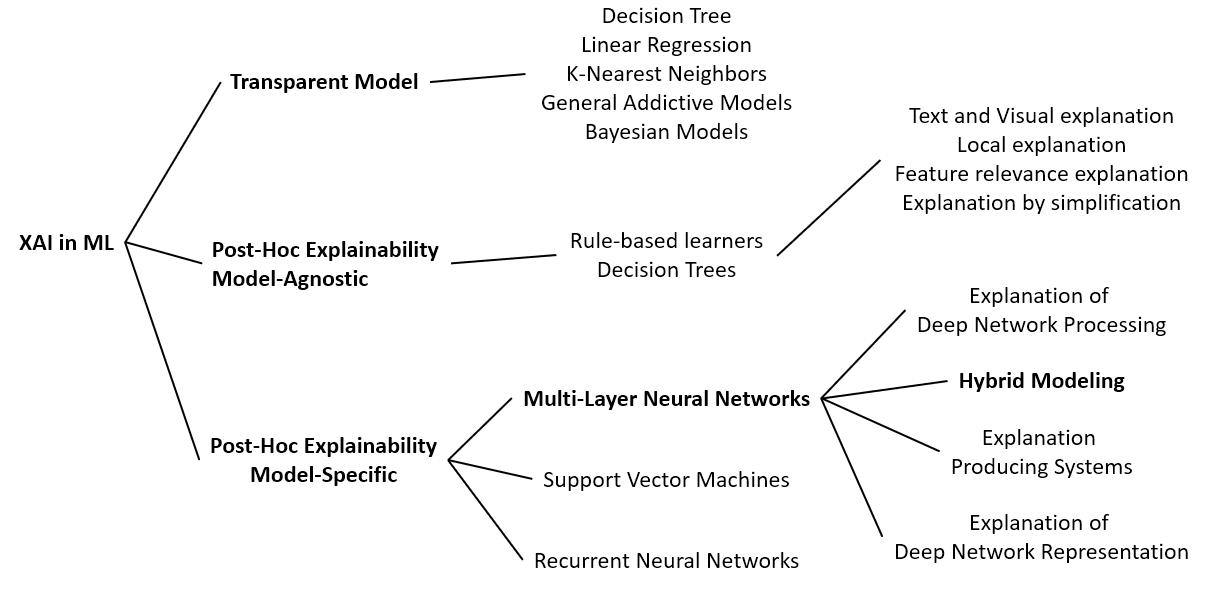
\includegraphics[width=1\textwidth]{bilder/Figure_4.png}
	\caption{Taxonomy for different XAI explainability techniques in ML models}
	\label{fig:Testbild}
\end{figure}

In contrast to transparent models, post-hoc explainable models are mostly black-box models, which need to use post-hoc techniques to extract and convert information from the model into understandable explainable content. Until now, it is introduced post-hoc techniques which are designed for these black-box models in general, which are local explanations, text explanations, visual explanations, feature relevance explanations, explanations by example and explanations by simplification. In addition, there are post-hoc techniques, which are specific developed and tailor-made for certain deep learning models, thus those methods can not be directly transferred to other models. In this survey, the hybrid modeling method is introduced combining transparent model with deep learning model in order to obtain insight and explanation of its prediction. In the next subsection, the various transparent models are described in details. 

\subsection{Transparent Model}
As introduced in the overview logistic regression model, linear regression model, K-nearest neighbors, rule-based learners, general addictive model and bayesian model are in the category of transparent model. In the following, a detailed description about their level of explainability is given.

\begin{itemize}
	\item \textbf{Linear/Logistic Regression Model}: This kind of machine learning model meet the three proprieties as defined earlier, which are algorithmic transparency, decomposability and thus simulatability. However, developer may use post-hoc explainability techniques in order to explain to non-expert users \cite{hosmer}. In addition, to maintain its simulatability, the size of such model must be limited. And its variables need to be understood from its developers and users. 
	\item \textbf{K-Nearest Neighbors}: KNN offers a simple solution to most of classification problems to developers. It is widely used in the area where explainability is required \cite{lli}. However, it is important before explaining and analyzing the prediction to understand its interpretable variable, which is the distance of different data points in the KNN case. Thus its explainability depends on the distance function, number of neighbors and used features. The usage of complex features and distance functions may make KNN not decomposable and only algorithmic transparent.
	\item \textbf{Rule-based Learners}: Every model that generates rules in order to learn data is rule-based learning. Rule-based learners are transparent models and are often used to explain complex opaque models by generating rules, thus explain the prediction being made. They are suitable to understand and explain other models given their inherent natural relation to human behaviour. However, when dealing with great amount of rules in a model or transferring conventional rules into fuzzy rules, the degree of explainability and the degree of interpretability are certainly reduced for better model performance \cite{langley}
	\item \textbf{General Addictive Model}: GAM is a collection of graphs, and each of graph represents the influence of a single variable. On the other hand the set of variables defines a set of smooth functions, for which it computes the prediction. These graphs can be linear or complex function, but inherently comprehensible, as each graph represents a variable. It allows users and developers to verify easily about the importance of each variable with regard to the predicted value. These models are understandable to make users feel confident and are already used in different disciplines related to risk assessment, healthcare, and energy etc. \cite{caruana, pierrot}. 
	\item \textbf{Bayesian Model}: The graphical property of Bayesian model provides users the probabilistic relationships between the feature and the predicted target and gives insight into set of variables regarding its conditional dependencies. Bayesian model is inherently algorithmically transparent and decomposable, which makes it simulatable. However, it can loss its decomposability and simulatability when introducing complex and highly abstract variables into the model \cite{cassandra}.
\end{itemize}

\subsection{Post-Hoc Techniques}
As stated in overview, post-hoc techniques are general methods, which are designed for any model using information extraction from its prediction. Some of the methods tend to visualize the model behavior, others simplify the model by introducing feature reduction and other complexity reduction methods. In the following, a detailed view of these techniques is discussed. 

\begin{itemize}
	\item \textbf{Text explanations}: It generates text or symbols that represent certain functions of the model in order to help explaining the results from the model. There are researches in which proposed generating text explanations from an image. Combining a Convolutional Neural Network (CNN) feature extractor with an Recurrent Neural Network (RNN) model to learn the meaning of image, and generating a text description of this image \cite{xu}. Overall the method is not widely used, because of the complexity of automatic text generation within an opaque system.
	\item \textbf{Visual explanations}: Visual explanations are essential in model explanation, as they help a black-box machine learning model to explain its input and output to its users and developers \cite{cortez}. Dimensionality reduction techniques are used to achieve interpretable simple visualization. However, to develop tool for visual explanation is a complex task, thus it is less common in the field of XAI. And almost all visualization methods can be combined with feature relevance techniques, in order to visualize the information to the end user.
	\item \textbf{Feature relevance explanations}: It aims to give an indication of the functions inside an opaque model by extracting features, measuring the influences of those features and variables in regard to predicted value. One important contribution is called SHapley Additive exPlanations (SHAP). It calculates a feature importance score for each predicted value with a set of desired properties \cite{lunberg}. Thus this method gives a relevance score for its variable and inner functions of a model and computes the sensitivity of the features in comparison of the predicted value. Feature relevance has became a popular method to develop XAI system, besides explanation by simplification.
	\item \textbf{Explanations by simplification}: The method is most broadly used technique under this category. Local explanations are also considered within explanations by simplification, since simplified models can only be extracted from part of a complex model. The most known technique is the Local Interpretable Model-Agnostic Explanations (LIME) \cite{ribeiros}. It builds linear models locally from set of predictions of an opaque model, in order to explain it. Another approach besides LIME is G-REX, which extracts rules from opaque models \cite{konig}. Both approaches set the popularity for using model simplification method to develop XAI system and will continue being explored in various fields of study.\cite{ribeiro, ribeiromt, mishra, johansson, johanssonu, ribeiros, konig}
\end{itemize}


\subsection{Hybrid Modeling}
Besides general post-hoc techniques, there exist also certain amount of works on tailor-made post-hoc techniques available, which are specific developed for certain deep learning models. One approach is the hybrid modeling method, shown in figure 5, where the authors tried to combine classical machine learning model KNN with its more complex opaque deep learning model: Deep Nearst Neighbors DkNN \cite{papernot}. The KNN model gives interpretable explanations of the predicted value, and tries to rationalize the DNN predicted value using evidence, namely a feature of confidence. In the work, it is called credibility which must supported by the training data.
\begin{figure}[htb]
	\centering 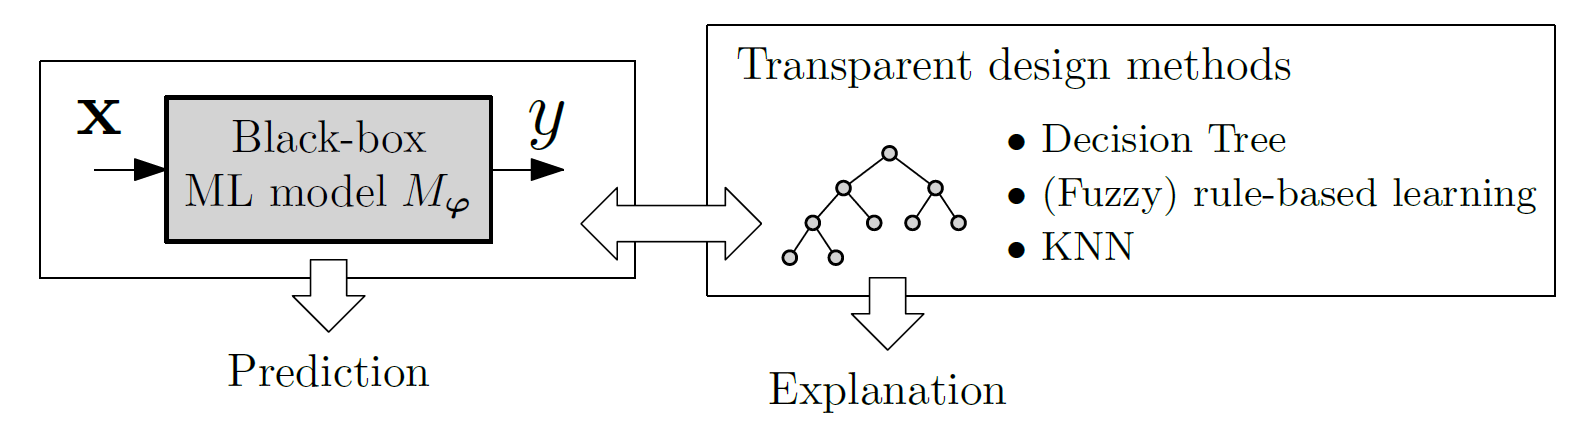
\includegraphics[width=0.7\textwidth]{bilder/Figure_5.png}
	\caption{Representation of hybrid modeling method \cite{aleja}.}
	\label{fig:Testbild}
\end{figure}

Another hybrid modeling approach is suggested in \cite{aamodt,caruanar}, where an opaque black-box system is map to a white-box model, that is more interpretable with a transparent case based reasoning (CBR) system. CBR system has the same intuition of reasoning as human, it tries to solve new problems by reusing solutions that were applied to similar problems from past. Both black-box DNN and white-box CBR are then paired with same simulation steps in order to improve model interpretability while maintaining the high model accuracy from DNN. Table 1 shows the available tools and libraries in XAI.

When developing an XAI system, there are no general procedure for an overall approach. Developers need to understand their needs and their target users in order to develop an XAI system which most fits their requirements and usages. A trade-off between interpretability and model performance is not always true, and can be avoided by applying correct AI model with XAI methods. A detailed discussion is given in the section under future of AI.

\begin{table}
	\begin{center}
	  \begin{tabular}{ |c|c|c| } 
		\hline
		\textbf{Tool} & \textbf{Programming language} & \textbf{ Functionality} \\
		\hline 
		ELI5 & Python & Debug ML classifiers and explain model predictions \\ 
		\hline
		What-If Tool & Python & \makecell{Developed by Google \\ It let user to understand a black-box classifier or regressor \\ easy-to-use interface \\ It can also visualize the results} \\ 
		\hline
		Yellowbrick & \makecell{Python \\ using scikit-learn API} & \makecell{Visual analysis and \\ diagnostic tools to facilitate machine learning model selection} \\ 
		\hline
		LIME & Python and R &  \makecell{Black-box model classifier explanations \\ able to explain image and text ML models and \\ outputs text explanations} \\ 
		\hline
		InterpretML & Python & \makecell{training interpretable models and \\ explaining black-box models, developed by Microsoft} \\ 
		\hline
		Lucid & Python Tensorflow & \makecell{A collection of infrastructure and tools \\ for research in neural network interpretability} \\ 
		\hline
		DALEX & Python and R & \makecell{Explore and explain any model's behaviour \\ uses local explanation around predictions\\ for classification and regression tasks} \\ 
		\hline
	  \end{tabular}
    \caption{\label{tab:table-name} Available tools and libraries in XAI}
    \end{center}
\end{table}

\section{A Use Case of XAI for Robot Task Planning}

\subsection{Motivations}
In this section, a use case for implementing XAI techniques is introduced, where the authors developed explainable and predictable plans for robot task planning \cite{zhang}. As the human-machine collaborations are growing nowadays, there exist potential safety risks when robot behave unexpected and harm the human operator. Nevertheless, human can interpret robot tasks differently while it is holding a cup or a knife, regardless the both motion and task planning is identical for robot. Thus the challenge lies in the human understanding of the robot model, which is inherently hidden and can be interpreted arbitrarily different. The goal of this paper is to enable robot naturally interact with human, it needs to explain the task it is currently operate on and also it's next plan step to the human operator in human-understandable labels, such as \emph{(picking up a cup)}, illustrated in figure 6. In order to achieve this, they trained a labeling model using conditional random fields method to compute its explainable plan with accurate predictions. In the following a detailed description of authors applied methods is discussed.  
\begin{figure}[htb]
	\centering 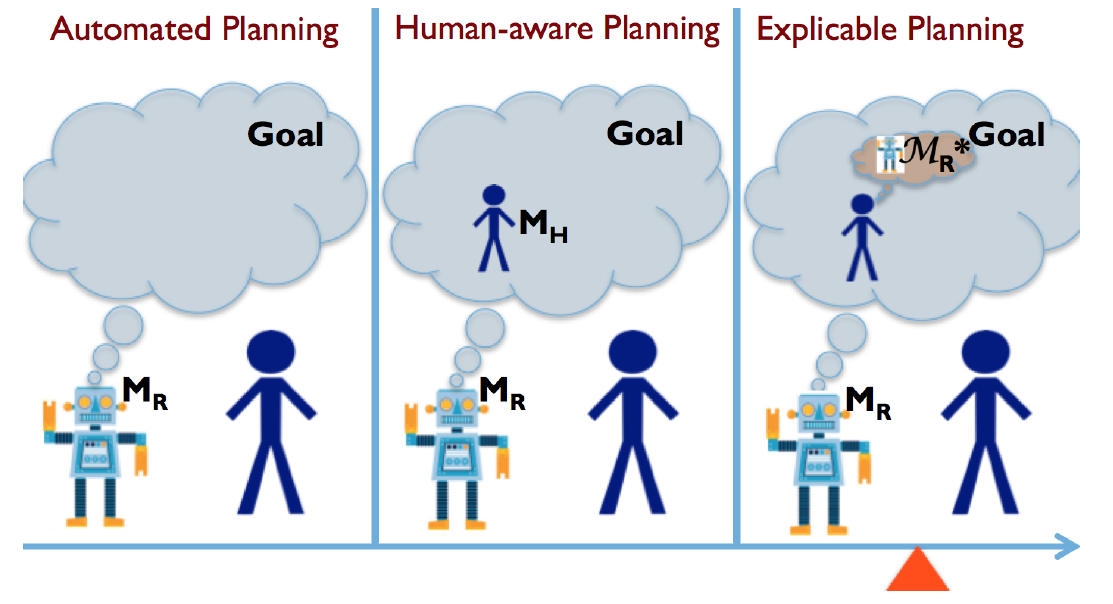
\includegraphics[width=0.5\textwidth]{bilder/Figure_6.png}
	\caption{Differences between automated task plannung, human-aware planning and explicable planning \cite{zhang}.}
	\label{fig:Testbild}
\end{figure}
\subsection{Applied Methods}
The problem is divided into two parts: explainability and predictability. First, the authors define the equation of finding such plan as: 
\begin{equation}
	\operatorname*{argmin}_{\pi_{M_R}} cost(\pi_{M_R}) + \alpha*dist(\pi_{M_R}, \pi_{M^*_{R}}) 
\end{equation}
where $\pi_{M_R}$ is the sequence of actions from the plan of the robot model $M_R$ and $\pi_{M^*_{R}}$ is constructed from the human's perspective of interpreted robot model $M^*_R$. $cost$ gives the cost of the plan, $dist$ computes the differences of two plans as distance and $\alpha$ is the relative weight factor for importance of explainability or predictability, which may vary in different circumstances. The assumption is made that their learning method can be directly approximate the distance values, such that:
\begin{equation}
	dist(\pi_{M_R}, \pi_{M^*_{R}}) = F \circ \mathcal{L^*}(\pi_{M_R})
\end{equation}
$F$ makes plan labels as input and $\mathcal{L^*}$ gives the labeling scheme from the model $M^*_R$, which can be trained and denote to $L$. The equation 1 now expands to:
\begin{equation}
	\operatorname*{argmin}_{\pi_{M_R}} cost(\pi_{M_R}) + \alpha * F \circ \mathcal{L}(\pi_{M_R}| \{S_i|S_i = \mathcal{L^*}(\pi^i_{M_R})\} )
\end{equation}
where ${S_i}$ is the set of training examples with the form of $(F_i, L^2_i)$, $F_i$ is the set of features for the action and $L^2_i$ is the one time-step further action label.

The explainability $\theta_{\pi_{M_R}}$ is thus computed by mapping the sequence of labels of robot action from $\pi_{M_R}$ into 0 or 1, where 0 is inexplainable when there is no label found, and 1 as explainable:
\begin{equation}
	F_{\theta}(L_{\pi}) = \frac{\sum_{i=[1,N]} 1_{L(\pi_i) \neq \emptyset}} {N}
\end{equation}
N is the length of such plan, $L(\pi_i)$ outputs the action label and $1_{formula}$ gives either 1 if the formula holds, or 0 otherwise.

Similar to explainability $\theta_{\pi_{M_R}}$, predictability $\beta_{\pi_{M_R}}$ is computed as following:
\begin{equation}
	F_{\beta}(L_{\pi}^2) = \frac{\sum_{i=[0,N]} 1_{|L(\pi_i)|=1} \wedge (1_{L^2(\pi_i)=L(\pi_j)} \vee 1_{L^2(\pi_{i:N}) = \emptyset})}  {N+1}
\end{equation}
$L^2_{\pi}$ is the sequence of labels with one predicted future time-step. Under the assumption that there is at most one task label for each current and future action. For $\pi_{j}$ with $j>i$, when the next predicted label of action $L^2_{\pi_i}$ has the same label of actual action $L_{\pi_j}$ or there is no further labels, which means the action of the robot has ended, it returns 1 for the current time-step. Thus $F_{\beta}(L_{\pi}^2)$ compute the ratio of all correctly predicted actions. Note that equations 4 and 5 can be extended for multiple task labels. Finally, they uses conditional random fields (CRFs) \cite{lafferty} to train and model the sequential labeling set and trained the examples using equation 3.
\subsection{A Concrete Example}
The above described learning method can be made more obvious, given the following example: Consider a rover has a goal of collecting boxes to a storage area of location $l_3$ and observe two locations $l_0$ and $l_6$ that contain the eye symbol, see figure 7
\begin{figure}[htb]
	\centering 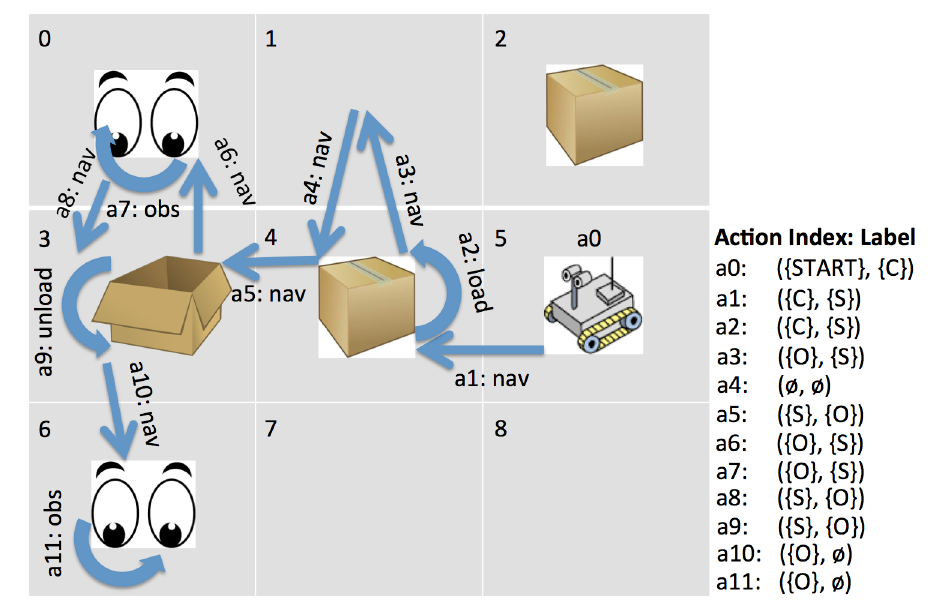
\includegraphics[width=0.5\textwidth]{bilder/Figure_7.png}
	\caption{A concrete example using labels to perform explainable and predictable plan \cite{zhang}.}
	\label{fig:Testbild}
\end{figure}

Following actions of such rover can be made: \{navigate $\l_{from}$ to $l_{to}$\}, \{observe $l$\}, \{load $l$\}, and \{unload $l$\} with $l$ as a location. It remains observed, if the location is once observed. Given three abstract tasks that can be understood from human operator: Collect (C), store (S) and observe (O). By starting from the initial location $l_5$, the rover should start and collect the resource from $l_4$, thus the label $a_0$ as (\{START\}, \{C\}) . Then in $a_1$ the rover navigates from $l_5$ to $l_4$ and collects the package. It outputs the action label as (\{C\}, \{S\}), same as in action $a_2$. In the next action $a_3$, it navigates unexpected to $l_1$, although it should perform store, but it can still be explained by labeling as (\{O\}, \{S\}), observed location $l_0$ and perform store action in the next state. However in $a_4$, the rover navigate back to the location $l_4$, which has no much meaning for human, since it is oscillating and performing redundant actions, hence the action is neither explainable nor predictable and is labeled as (\{$\emptyset$\}, \{$\emptyset$\}). The same procedure of explanations and predictions can be made until the end of the plan, after the rover has stored the package in $l_3$ and observed the two locations $l_0$ and $l_6$.
\subsection{Conclusion}
In the paper, the authors evaluate further their methods with other learning methods and plan synthesis with respect to explainable and predictable plans. And they conclude that one of their implemented method gives the best overall results of high explainability with accurate predictions in their experiments. In outlook, the authors mentioned that it can be further developed using other complex learning approaches and use the techniques in military defense applications.
\section{Future of XAI}

\subsection{Principles of AI}
It is time to sum up the concept of XAI within the context of AI, in order to create a holistic understanding toward better developed AI system and other criteria surrounding it. In this section, a detailed look into principles and guidelines of developing such AI system combing XAI methods is discussed. Different companies and governments have addressed various principles of AI under their own understanding, most of them do not differ much. In the following, 3 selected statements are shown:

\begin{center}\emph{"We will design AI systems that provide appropriate opportunities for feedback, relevant explanations, and appeal. Our AI technologies will be subject to appropriate human direction and control." -  Google Our Principles} \cite{google}\end{center}

\begin{center}\emph{"The data, system and AI business models should be transparent. Traceability mechanisms can help achieving this. Moreover, AI systems and their decisions should be explained in a manner adapted to the stakeholder concerned. humans need to be aware that they are interacting with an AI system, and must be informed of the system's capabilities and limitations." - EU high level Expert Group on AI} \cite{eu}\end{center}

\begin{center}\emph{"Designing AI to be trustworthy requires creating solutions that reflect ethical principles that are deeply rooted in important and timeless values. ... AI systems should be understandable." - Microsoft Our Approach to AI} \cite{microsoft}\end{center}

From the above statements one can conclude that forms of explainability, transparency, accountability and ethical principles need to be addressed and featured in an AI system, in order to fulfill their requirements and responsibilities when using such system, which also indicates that only using XAI methods to gain explainability of a black-box model might not be enough. One must elaborate and cover all those principles into AI system, and such concept is called Responsible AI. 

There are 4 major methodological steps when designing such AI system \cite{leslie}:

\begin{enumerate}
	\item Domain specific knowledge need to be taken into account when developing such explainable, accountable AI system. The developer should understand the purpose of building such system and offer such explanations and reasoning by which the end users are required. In addition, interpretability of such technologies and methods used in the AI system is also given by the developer. 
	\item Use transparent and interpretable models whenever possible. Complex and opaque black-box model is not always preferred, regarding to their high accuracy and advanced performance. The decision of which AI methods and XAI techniques should be chosen with domain specific needs and risks. With transparency and explainability in hand, one can then develop more sophisticated opaque models in order to gain higher performance from existing system.  
	\item When an opaque black-box system is unavoidable, the notion of fairness, safety and interpretability need to be translated as features into such system, in order to weight the related concepts as impacts toward predicted value. An evaluation metrics should be developed underlining those abstract notions and need to be quantified. And such design of metric have to be evaluated by comparing with other XAI tools that provide a level of explainability in the similar field of study.   
	\item Finally, one should understand the limitations, capacities and cognitive skills of indiviuals when developing such AI system. It should give answers as a human-like system, not necessarily to think and perform as the end-user, but in a way such mental models of human, necessary vocabulary from domain specific knowledge and other means of logical and reasonable predicted results under the frame of expertise should be considered and implemented in the AI system. 
\end{enumerate}

\subsection{Challenges}
There are several challenges in an XAI system: First, explanations are not necessarily reliable. If an AI system produces a convincing but misleading and incorrect explanations, users and developers might gain a false confidence and trust the system blindly without being justified. This transparency and explanability is double-edged, as research shows that users give great trust in transparent models even when they are wrong and ought not to be trusted \cite{sangdeh}. It can also be easily misused by generating false interpretations to fool or manipulate people, such as targeted advertising on social media \cite{andreou}.

By developing an XAI system may also introduce ambiguities. In the EU General Data Protection Regulation (GDPR) states that explanations need to be required for non-technical expertise, which may introduce such ambiguities and misunderstanding for policy makers, politicians and law makers \cite{wachter}. For instance, the concept of reasoning is subjective and it is completely dependent on the users and how they reason the idea on their own and see the XAI system as reasonable, the same notion goes to explanation. As described in section 2.2, different users require different forms of explanations in various contexts for their own expertise. Therefore the demand of such XAI system may vary greatly and the design of such system is determined to be tailor-made. 

It is also worth mentioning that constrictive explanation is better, which means explanation should not only about why the predicted value is such, but also why it make this choice rather than other predictions. Nevertheless, it is also shown that the use of counterfactual in explanations can help the end-user to better understand the decision of an opaque model \cite{byrne}. 

Another one is the performance-accuracy trade-off for XAI system. It needs to keep relatively simple to be interpretable, and therefore lose its previous high accuracy. This can be overcome using hybrid modeling method, which was discussed in the section 3.4. Also certain subject such as autonomous driving, cancer detection are highly mathematical in nature and cannot be interpreted in any natural language, regarding to the vagueness and ambiguity it provides. 

Finally, the explainability of an AI system is inherently limited by the random sample of data it used. With these challenges in mind, researchers and developers give birth to the concept of responsible AI, a hierarchical concept that adopts several AI principles and goes beyond explainability.

\subsection{Opportunities}
Although the performance-accuracy trade-off can occur in ML models, however one can improve such trade-off between model interpretability and performance in means of hybrid modelling approaches and other new post-hoc explainability techniques, so that the model does not suffer oversimplification while maintaining essential features, illustrated in figure 8.

\begin{figure}[htb]
	\centering 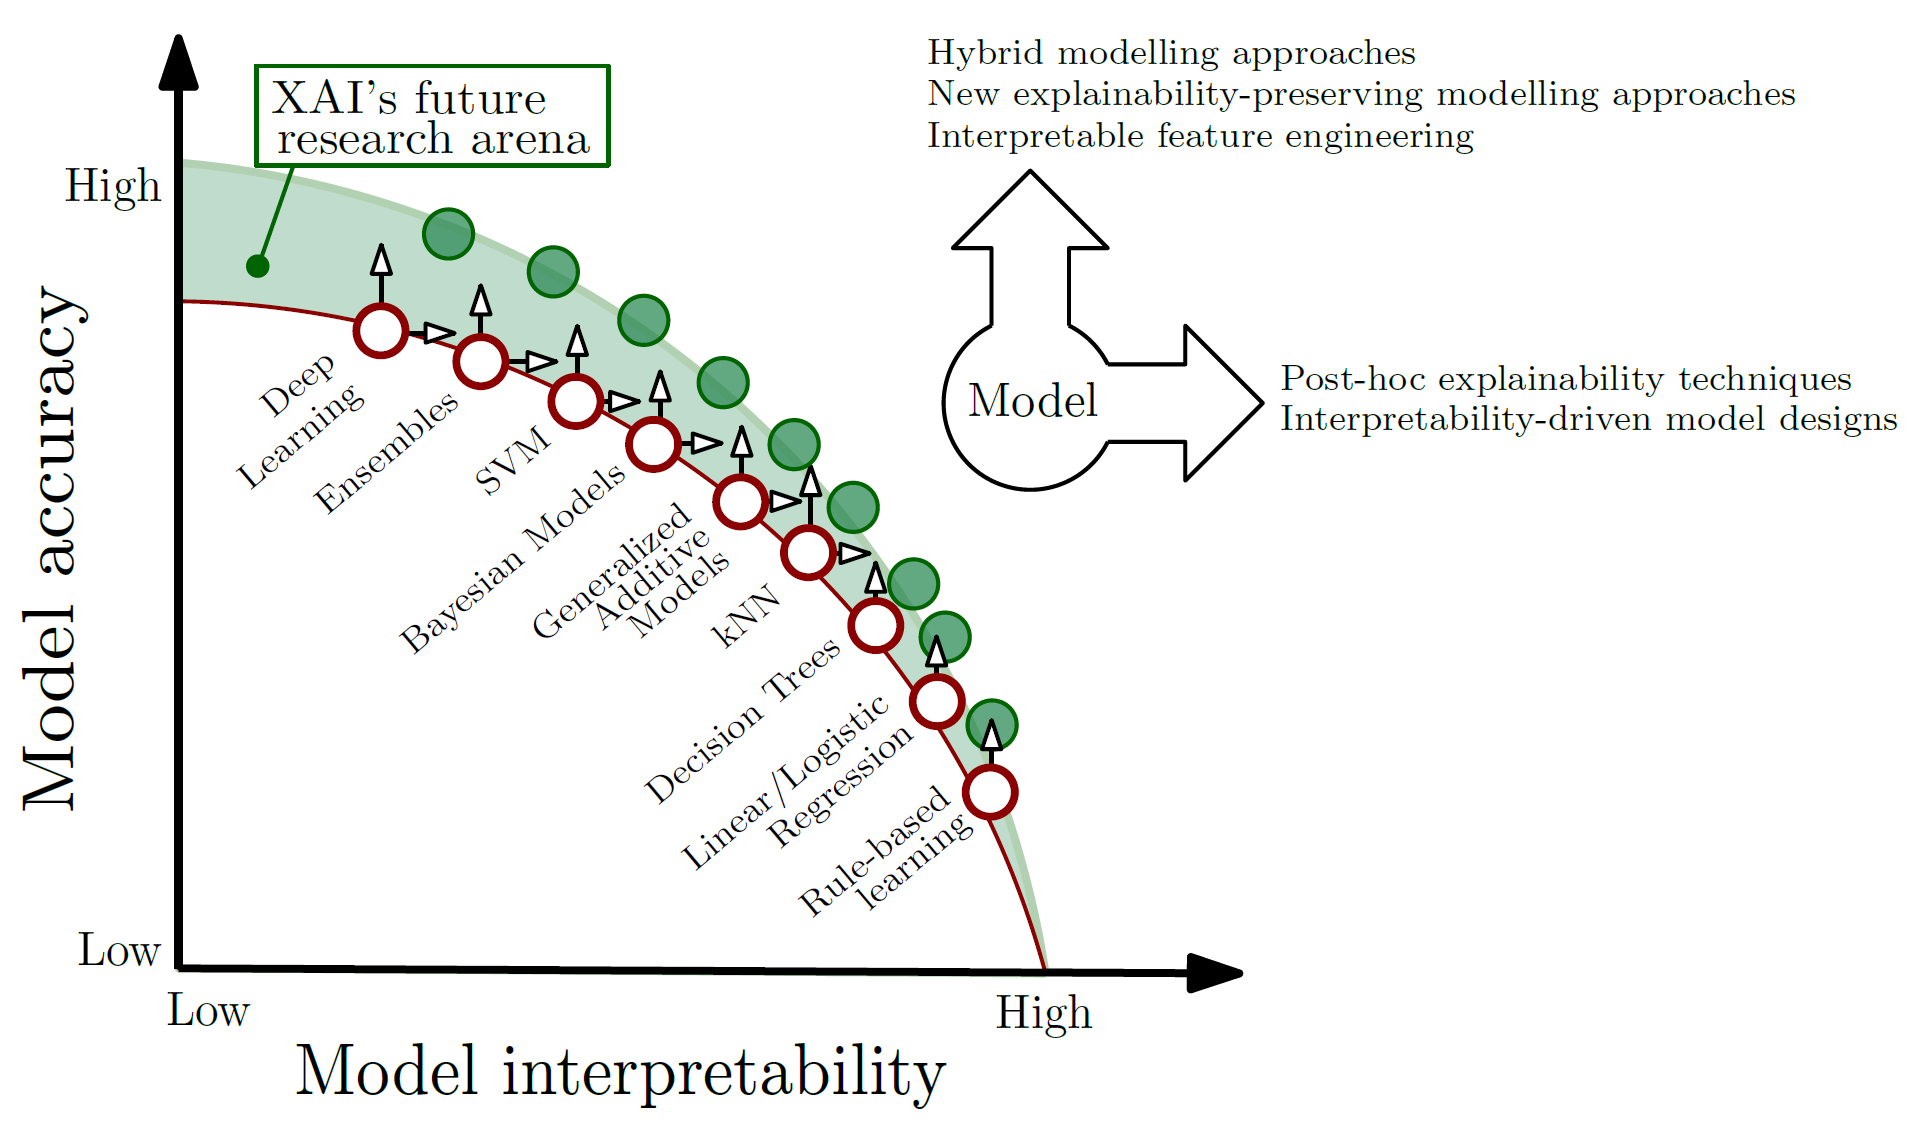
\includegraphics[width=1\textwidth]{bilder/Figure_8.png}
	\caption{Trade-off between model interpretability and performance \cite{aleja}.}
	\label{fig:Testbild}
\end{figure}

Furthermore, one can develop a general purpose metrics evaluation that makes the function of such AI system and underlining explanation clearer to the end-user. The evaluation metric should include the goodness of fit, degree of usefulness and degree of satisfaction of such explanations. Moreover in order to improve the explanation, a mental model of the end-user need to be conducted. There are several existing evaluation methods, which can make the AI system and XAI methods more convincing and understandable to end-user, such as goodness checklist, elicitation methods for mental models, explanation satisfaction scale, explanation trustworthiness and model reliability \cite{hoffmann, mohseni}. 

Lack of general vocabulary and different definitions around XAI can be seen as a challenge as well as opportunity, as in the early day in the field of XAI. It gives developer a large degree of freedom to conduct their research interests in XAI without constraint in sophisticated technical vocabulary. However, an overall understanding of general evaluation on how comprehensible such explanation and interpretation are made is necessary for end-users with different fields, experts or non-experts. An objective metrics to evaluate the capability of XAI in an AI system is well needed in order to make constant progress and visualize such improvements in this field. One suggestion is to use knowledge from psychology, cognitive sciences to create convincing but objective explanations to the end-user \cite{hoffmann, mohseni}.

\section{Conclusion and Outlook}

This survey gives an overview of XAI and its techniques to empowering AI system into transparent, interpretable system. In the section of future of XAI, it is concluded that explainability may not enough and will need to develop responsible AI, which shares features of sustainability, privacy and accountability while harnessing the potential of XAI with the degree of explainability in applied AI system. The goal is to create predictive responsible AI that are on the one hand highly accurate, and on the other hand highly interpretable, that one can use for trustworthy decision making. The quote from Arvind Narayanan, computer science professor of Princeton gives this remark and warning of the underlining risks when deploying a AI black-box system, without knowing exact object functions and feature extractions inside such system:

\begin{center}\emph{"Contrary to the 'tech moves too fast for society to keep up' clich�, commercial deployments of tech often move glacially? Just look at the banking and airline mainframes still running. machine learning models being trained today might still be in production in 50 years, and that is terrifying."} \cite{arvind}\end{center}

Engineering is inseparable from human norms, human values and human society, it is always about cooperation and collaboration with others. As developing and deploying an AI system falls into the realm of engineering, one can conclude that in aspects of sustainability, privacy, equality and accountability, the goal is essentially to develop a more responsible use of AI, a path toward Responsible AI. 







